%&pdflatex
\documentclass[12pt]{article}


\usepackage{graphicx}
\usepackage{colortbl}
\usepackage{xr}
\usepackage{longtable}
\usepackage{xfrac}
\usepackage{tabularx}
\usepackage{booktabs}
\usepackage{hyperref}
\usepackage{xcolor} % for different colour comments
\usepackage{fullpage}
\newcounter{rowcount}
\setcounter{rowcount}{0}

%
%\hypersetup{
%    bookmarks=true,         % show bookmarks bar?
%    colorlinks=true,        % false: boxed links; true: colored links
%    linkcolor=black,        % color of internal links (change box color with linkbordercolor)
%    citecolor=green,        % color of links to bibliography
%    filecolor=magenta,      % color of file links
%    urlcolor=cyan           % color of external links
%}

%% Comments
\newif\ifcomments\commentstrue
\ifcomments
\newcommand{\authornote}[3]{\textcolor{#1}{[#3 ---#2]}}
\newcommand{\todo}[1]{\textcolor{red}{[TODO: #1]}}
\else
\newcommand{\authornote}[3]{}
\newcommand{\todo}[1]{}
\fi
\newcommand{\wss}[1]{\authornote{magenta}{SS}{#1}}
\newcommand{\ds}[1]{\authornote{blue}{DS}{#1}}
\newcommand{\kly}[1]{\authornote{green}{KL}{#1}}
\newcommand{\cc}[1]{\authornote{orange}{CC}{#1}}

%%%%%%%%%%%%%%%%%%%%%%%%%%%%%

\begin{document}

\title{Design Document for Quarters}
\author{Team 6\\ \\James Anthony (anthonjb)\\ Wenqiang Chen (chenw25)\\ Carolyn Chong
(chongce)\\ Kevin Ly (lyk2)}
\date{\today}

\maketitle

\pagebreak

\tableofcontents

\section*{Revision History}
\begin{tabular}{|c|c|}
\hline
\textbf{Date}  & \textbf{Comments} \\ \hline
January 5, 2016 & Created first draft. \\
\hline
\end{tabular}

\pagebreak

%%%%%%%%%%%%%%%%%%%%%%%%%%%%%

%Introduction and Overview
\section{Introduction and Overview}

\subsection{Document Structure}
This document provides insight as to how Quarters was built. Design principles are stated followed by a list of anticipated and unlikely changes. The web application's system architecture is then decomposed and the design details explained based on the Software Requirements Specifications (SRS) document. Lastly, error handling is discussed and a project schedule is presented.

\subsection{Design Principles}
TBC. includes a clear statement of what design principle(s) is (are)being used. The web application was designed in a XXX manner. This was to ensure XXX. Decomposition follows the design principle suggested for the design. In many cases the appropriate design principle will be design for change (information hiding). Methodologies include top-down, bottom-up, stepwise refinement, prototyping, modular, or object-oriented.


%Connection between requirements and design
\section{Connection between requirements and design}
what design decisions needed to be made torealize the requirements – for instance, if there are security NFRs, what decision is made onhow to do this – password protection?

%Anticipated Changes
\section{Anticipated Changes}
\begin{enumerate}
\item{}
\end{enumerate}

%System Tests
\section{Unlikely Changes}
\begin{enumerate}
\item{}
\end{enumerate}

%
\section{Decomposition into Components}

%
\section{Uses hierarchy, or control flow diagram, or inheritance graph}

%
\section{Traceability from requirements to design components}

%
\section{Traceability for anticipated changes to components}

%
\section{Error Handling}

%
\section{User interface elements descriptions}

%
\section{Overview of key algorithms}

\clearpage
%
\section{Relational database structure}
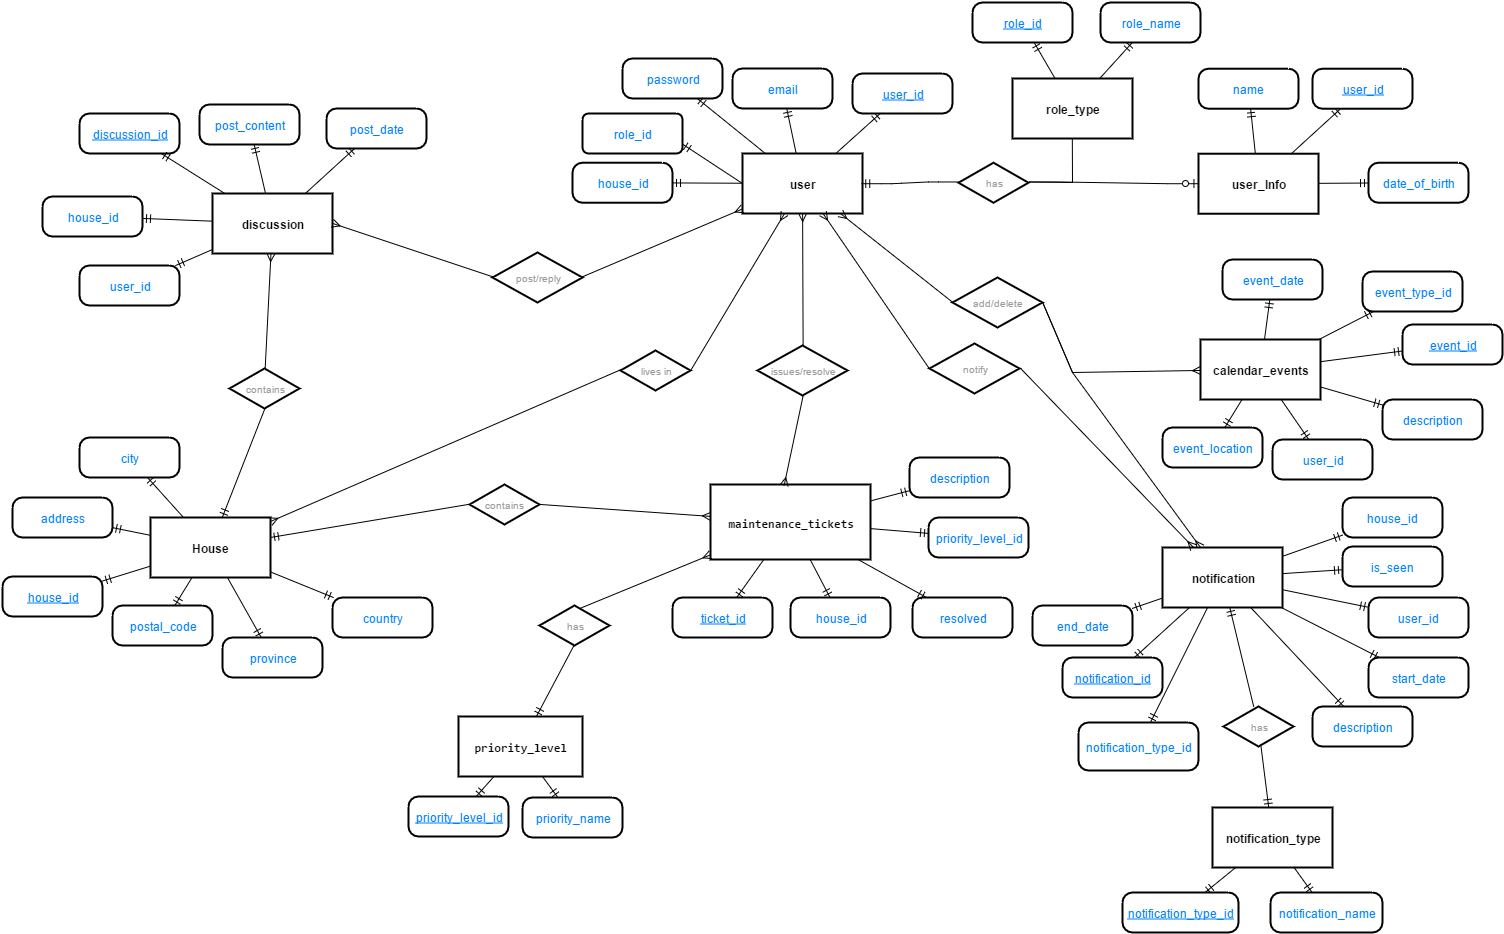
\includegraphics[scale=0.397, angle=-90, keepaspectratio]{images/ER_Diagram.png}
%
\section{Communication protocols specified}

%
\section{Description of each component, or UI element, or database table}

%
\section{Development Details}
\begin{description}
  \item[Languages of implementation] \hfill
    \begin{itemize}
      \item NodeJS [1]
      \item PostgreSQL [2]
      \item Jade [3]
    \end{itemize}
  \item[Supporting frameworks] \hfill
    \begin{itemize}
      \item Bootstrap [4]
      \item ExpressJS [5]
    \end{itemize}
  \item[Supporting technology] \hfill
    \begin{itemize}
      \item Ubuntu Server [6]
    \end{itemize}
\end{description}

%
\section{GanttProject shows a detailed project schedule}

%
\section{Pert chart shows dependencies}

%
\section{References}
\begin{description}
  \item[[1]] link
  \item[[2]] link
\end{description}
\end{document}
